\documentclass[sigchi, review, anonymous]{acmart}

\usepackage{booktabs} % For formal tables


% Copyright
\setcopyright{none}
%\setcopyright{acmcopyright}
%\setcopyright{acmlicensed}
%\setcopyright{rightsretained}
%\setcopyright{usgov}
%\setcopyright{usgovmixed}
%\setcopyright{cagov}
%\setcopyright{licensedcagov}
%\setcopyright{cagovmixed}
%\setcopyright{licensedothergov}

% DOI
%\acmDOI{10.475/123_4}

% ISBN
%\acmISBN{123-4567-24-567/08/06}

%Conference
\acmConference[Submitted to CHI'19]{ACM SIGCHI Conference}{May 2019}{Glasgow, UK}
%\acmYear{1997}
%\copyrightyear{2018}

%\acmPrice{15.00}


\begin{document}
\title["Who's There?": A Wearable Device to Identify Others]{"Who's There?": A Wearable  Device to Help Visually Impaired Users Identify Others}
%\titlenote{Produces the permission block, and
%  copyright information}
%\subtitle{Extended Abstract}
%\subtitlenote{The full version of the author's guide is available as
%  \texttt{acmart.pdf} document}

\author{Srishti Palani}
\authornote{Currently at the University of California, San Diego, Cognitive Science Department}
%\orcid{1234-5678-9012}
\affiliation{%
  \institution{Mount Holyoke College}
}
\email{palan22s@mtholyoke.edu}

\author{Barbara Lerner}
\affiliation{%
  \institution{Mount Holyoke College}
  \streetaddress{50 College Street}
  \city{South Hadley}
  \state{MA}
  \postcode{01075}
}
\email{blerner@mtholyoke.edu}


% The default list of authors is too long for headers.
%\renewcommand{\shortauthors}{B. Trovato et al.}


\begin{abstract}
Approximately 4\% of our world's population is visually impaired, with 65\% of them over age 50. Visual impairment often leads to a loss in independence and diminished sociability, which in turn reduces life satisfaction. Interacting with visually-impaired users, we identified three specific problems: difficulty recognizing those in their surroundings; inability to proactively greet persons entering their social space; and not knowing if the person they are interacting with is within hearing range as they move around. In this paper, we describe a single-purpose, wearable bracelet with sonifications and vibro-tactile communication that provides low-cost and intuitive assistance to help visually impaired users identify and place potential interactors in their surroundings.  This project presents a first step in the design of intuitive audio-haptic devices that might benefit not just the visually-impaired, but also people with memory challenges or difficulty recognizing faces.
\end{abstract}

%
% The code below should be generated by the tool at
% http://dl.acm.org/ccs.cfm
% Please copy and paste the code instead of the example below.
%
 \begin{CCSXML}
<ccs2012>
<concept>
<concept_id>10003120.10011738.10011775</concept_id>
<concept_desc>Human-centered computing~Accessibility technologies</concept_desc>
<concept_significance>500</concept_significance>
</concept>
<concept>
<concept_id>10003120.10003138.10003141</concept_id>
<concept_desc>Human-centered computing~Ubiquitous and mobile devices</concept_desc>
<concept_significance>300</concept_significance>
</concept>
<concept>
<concept_id>10003456.10010927.10003616</concept_id>
<concept_desc>Social and professional topics~People with disabilities</concept_desc>
<concept_significance>300</concept_significance>
</concept>
</ccs2012>
\end{CCSXML}

\ccsdesc[500]{Human-centered computing~Accessibility technologies}
\ccsdesc[300]{Human-centered computing~Ubiquitous and mobile devices}
\ccsdesc[300]{Social and professional topics~People with disabilities}

\keywords{Visually-impaired, Assistive Technology}

%\begin{teaserfigure}
%  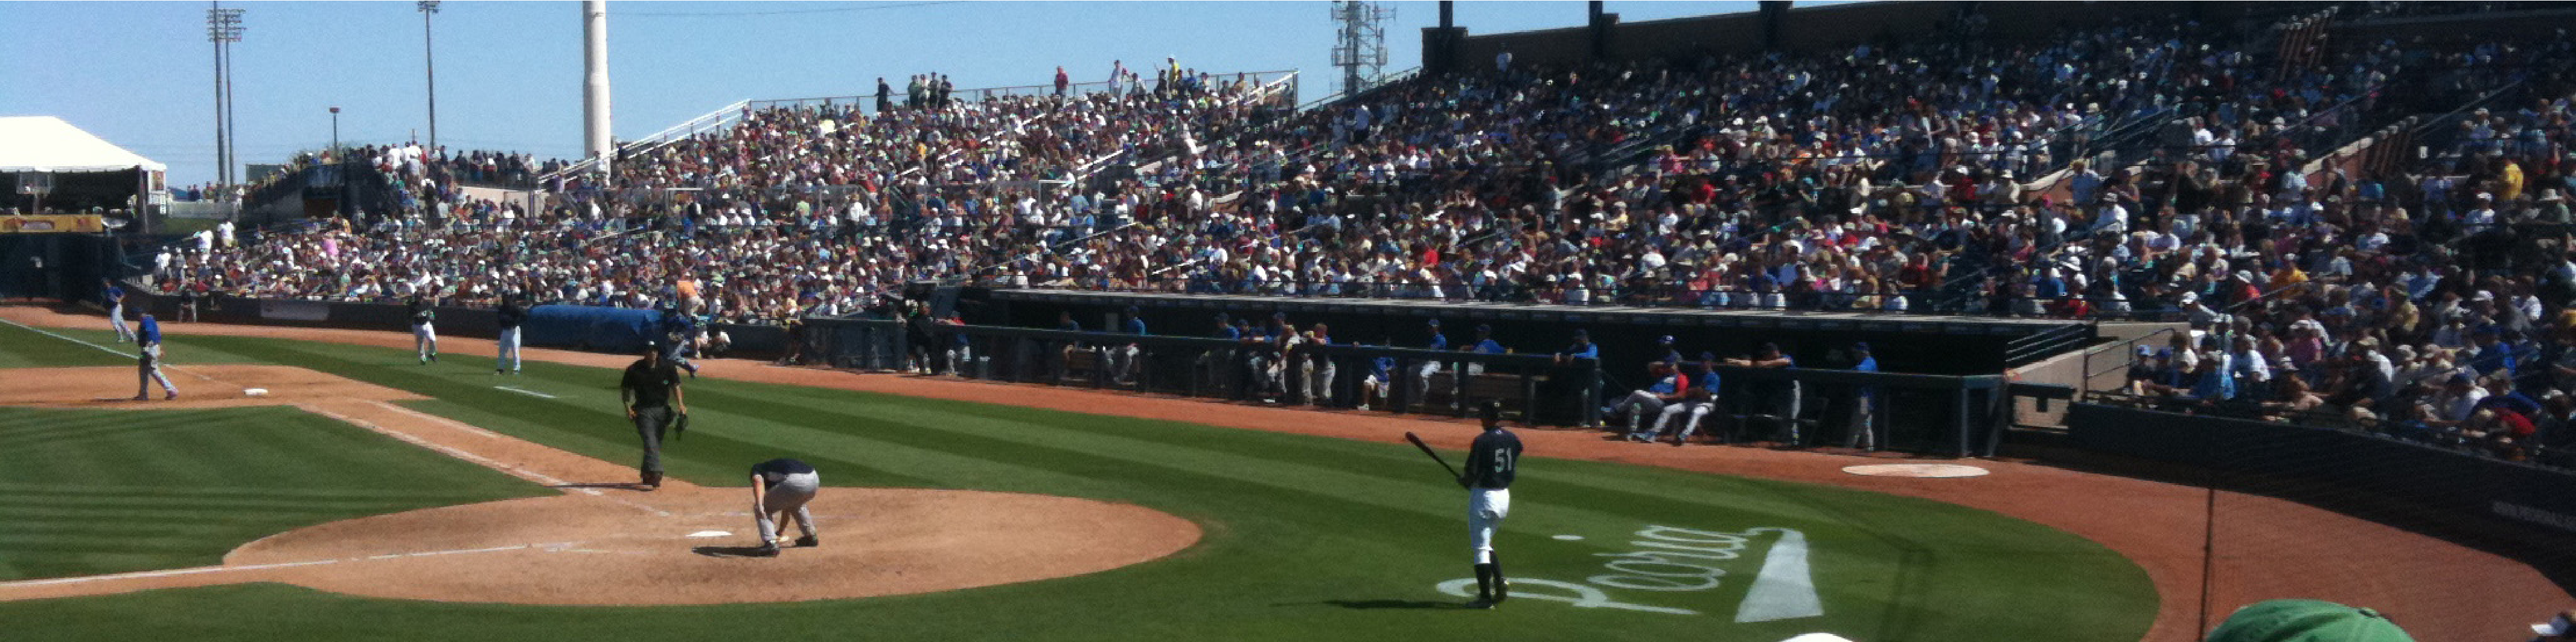
\includegraphics[width=\textwidth]{sampleteaser}
%  \caption{This is a teaser}
%  \label{fig:teaser}
%\end{teaserfigure}


\maketitle

\section{Introduction}
% * <blerner@mtholyoke.edu> 2018-09-12T15:51:08.443Z:
% 
% This is the abstract from your thesis.  We will want to change it to better fit the content of this paper.
% 
% ^.
Approximately 4\% of the world's population has a reduced ability to see that can not be cured by standard corrective measures such as glasses or even surgery. 65\% of visually impaired over age 50; and an estimate of 90\% of them live in low and middle-income countries. While these numbers are shocking, the bigger challenge is the reduced confidence and life satisfaction that the visually impaired experience as a result of loss in independence and diminished sociability. Interacting with visually-impaired people and their family and friends, we identified three specific problems that they face while communicating with others independently: 
\begin{itemize}
\item difficulty recognizing those in their surroundings;
\item inability to proactively greet persons entering their social space;
\item and not knowing if the person they are interacting with is within hearing range as they move around.
\end{itemize}
Our goal in this research project is to design an assistive device for the visually impaired that helps them identify and place persons in their surroundings such that it increases their sociability and independence.

Most of the work done so far in the technological research community to support the independence and social inclusion of the visually impaired is done by enabling smoother navigation. While technologists continue to work to improve accuracy, security and making these technologies more accessible at a low cost to visually impaired users, these devices only detect stationary objects that are part of the environment. There has been no significant research done towards recognizing and placing other people in the user's environment. Developing a usable solution to this problem requires not just developing the technology, but also understanding this as a cognitive and social problem, where the solution must organically add to the mental and social schemas already learned by the blind user. 

In this project, we approached this socio-technical problem by employing a systems approach to understand the cognitive, social and technical sides and then built a focused solution using a user-centered design approach. First, we researched the neuro-cognitive background of visual impairment and adaptation and then we looked at the technological background in creating assistive technology, and multi-sensory user interfaces. As part of the user-centered design approach, surveys and semi-structured interviews were used to understand and identify explicit user needs and wants. We also employed the Think-Aloud Protocol to evaluate user feedback during usability testing and gain insight into the users' cognitive processes, comfort levels and feelings while they interact with the device and performing various structured tasks. Additionally, we used a rubric to track the users' independence in engaging with social tasks while using the device.

Using the iterative user-centered design process, we developed two distinct prototypes with several iterations of the design-thinking process. The first relied on an iPhone to notify the user of who was where in their surroundings through designated speech notifications, sonifications and vibro-tactile haptic notifications. While it performed the tasks, it was too cognitively overwhelming, frustrating and exhausting for a blind user because of the phone's many notifications and functions. Therefore, it was ineffective in organically augmenting their perception of who was in their surroundings.

Our second prototype, described in this paper, incorporates three techniques: building a smart environment; designing a single-purpose, wearable bracelet with sonifications and vibro-tactile communication; and creating a novel audio-haptic user interface. We evaluated this device and chose it as our current solution because it is a low-cost, low-energy, easy-to-use, intuitive device that was successfully used by potential users to identify and place potential interactors in their surroundings during usability testing and user feedback sessions. 

This project shows us a way that we can overcome the challenges of socio-technical problems to contribute something significant to not only the field of assistive technology, but also to the field of multi-sensory augmentation in human-computer interaction. It expands on the visually-impaired user experience with technology and the pain points so that we can build more intuitive technology for this large subset of people. Furthermore, it presents a foundation for designing audio-haptic interfaces and devices for not only visually-impaired, but also for those with other age-related problems such as memory loss (dementia), trouble recognizing faces (prosopagnosia) or even problems with depth perception.

In Section \ref{sect:background}, we describe related work in assistive technology design and understand the users' cognitive, social and technological needs. Section \ref{sect:wearable} describes the hardware and software design of the wearable device.  Section \ref{sect:evaluation} discusses usability testing and user feedback. We conclude in Section \ref{sect:conclusion} with a discussion of the lessons learned, limitations and future directions.

\section{Related Work: Understanding Visually-Impaired Users' Needs}
\label{sect:background}
\subsection{Understanding Existing Assistive Technology}
Most of the work done so far in the technological research community to support the independence and social inclusion of the visually impaired has been done to enable smoother navigation. Assistive technology has been extensively researched and created for both outdoor and indoor navigation by identifying objects, barriers and, entryways, including \cite{Bousbia-Salah:2007ab,Chumkamon:2008ab,Ivanov:2012ab,Ladetto:2002aa,Loomis:2006aa,Makino:1996ab,Ran:2004ab}. Where outdoor systems rely upon GPS to locate the user \cite{Loomis:2006aa,Makino:1996ab,Newman:2002aa}, indoor systems typically rely upon physical augmentation of the environment such as ultrasound \cite{Bousbia-Salah:2007ab,Ram:1998ab,Runge:2011aa}, Wi-Fi access points \cite{Evennou:2006:AIW:1288263.1288407,Rajamaki:2007aa}, radio frequency identifier (RFID) tags \cite{Chumkamon:2008ab,Na:2006aa,Willis:2004aa} or expensive sensing equipment such as computer vision \cite{Golding:1999ab,Ran:2004ab}   or  integrated systems modeling the input from a combination of these \cite{Yelamarthi:2010ab}. 

Since we want to make this device as usable as possible, we need it to be a low-cost, low-energy system that can flexibly map surroundings and reliably identify people with as little need for pre-existing architecture as possible. These requirements eliminate the possibility of using the technology described above.

There are a few recent research papers published that use Bluetooth Low Energy (BLE) beacons embedded in the environment and smart phone technology to help the blind with indoor navigation \cite{ahmetovic2016navcog, Duarte-K.:2014aa}. NavCog built by a team led by Dragan Ahmetovic at Carnegie Mellon University \cite{ahmetovic2016navcog} is a low-cost low-energy mobile application that provides turn-by-turn navigation assistance based on accurate real-time localization over large spaces from Bluetooth Low-Energy beacons placed in the environment. It is useful in guiding visually-impaired users in unfamiliar and complex environments. While its focus is still on avoiding static objects during navigation rather than social interaction, it demonstrates the use of low-cost, low-energy equipment in navigation.  

A few studies also used Near Field Communication (NFC) or a system pulling from multiple sensors in real time to build a semantic-rich interior model of a building so that it is useful for navigation. An example of such a navigation application is RSNAVI, built by Rosen Ivanov \cite{Ivanov:2012ab}.  It is a context-aware indoor navigation system that uses information from RFID tags, and other sensors planted on the static surfaces of a building to build a semantic-rich interior model of the building and provides the user with step-by-step instructions on how to navigate the space in real-time. This is a very impressive system that does well to help the user navigate an indoor environment, but does not provide any information about other people inside the environment with whom the user could engage. 

Overall, these solutions do not help answer our research question of identifying and placing \textit{people} in the user's surroundings. These applications were designed for navigation around static objects such as walls, barriers, and objects. In our research problem not only  is the user moving, but the potential interactors are also moving  in the environment making it different and more dynamic. 

\subsection{Understanding How Visually Impaired Users Create Mental Maps}
In order to augment the blind user's perception of who is in their surroundings, we need to first understand how their mind perceives and processes the space around them. Most of the information required for mapping is gathered through the visual channel \cite{lynch1960image}. In the absence of this visual information, the blind adapt to create mental maps through compensatory sensory channels such as touch, sound and even language \cite{jacobson1993art,bavelier2002cross,roder2001auditory,petitto2000speech,liotti1998auditory,leclerc2000brain,kujala1995visual}. This phenomenon is known as \textit{cross-modal plasticity}\cite {bavelier2002cross}.

The blind develop cross modal plasticity to reroute auditory and tactile information to create mental imagery and maps of their surroundings. There are certain differences in how cross modal plasticity develops. Congenitally blind individuals or individuals with early-onset blindness are more perceptive to changes in the auditory and tactile cues, which enables them to create more accurate mental maps than those who experience late onset blindness \cite{ptito2008alterations}.

Current work to develop intuitive user interfaces builds on this information by employing either speech notifications, sonifications or haptic notifications. Speech notifications are essentially talking signs attached to static objects. Sonifications are used to help map the environment by associating different materials or objects with differences in frequency, amplitude or timbre of the sound \cite{brock2013supporting,massof2003auditory,striem2014visual}. The use of haptic user interfaces is more recent and is used by tactile graphic displays by modulating the pressure and frequency to create a recognition \cite{lahav2008haptic,belardinelli2009sonification}. However, haptic interfaces have very low resolution because it is hard to differentiate between and learn too many haptic cues \cite{lahav2008haptic}. 
% Furthermore, while designing sonic and tactile  notifications in user interface, we must be cautious to prevent sensory adaptation over a period of time. 

\subsection{Understanding Use of Interpersonal Space}
To understand the social aspect of how we use the space around us to interact with people we look at the interpersonal space model proposed by Edward Hall in 1963 \cite{hall1963system}. This models states that the way we interact with people changes depending on how far away they are from us and classifies interpersonal space into four distinct zones: (i) intimate space, (ii) personal space, (iii) social space, and (iv) public space.

Intimate space, within about 1.5 feet, is generally used for confidential or really close interactions such as embracing, touching or whispering. Personal distance,  1.5 to 4 feet, is generally only entered by close friends and family.  Social space, 4-12 feet, is the distance at which other people are generally acknowledged and greeted. These might be people in the same room or walking down the hallway, but are not engaged in a long conversation. Lastly, there is the public space, where other people are present but not generally interacted with, such as at a public gathering, like a concert. 

\subsection{Understanding Technology Used Every Day }
Based on the technological literature review and our understanding of the social and cognitive background we developed an initial prototype that was an iPhone application. The iPhone notified the user of who was where in their surroundings through speech notifications, sonifications and haptic notifications. The application could detect and keep track of multiple people in the user's surroundings.  In evaluating this prototype with a participant who had experienced late-onset blindness and had no light perception, the user found the device to be unintuitive and cognitively overwhelming. This was because not only was the user being notified of where others were in their space, they were being notified of calls, texts, and other information,. 

In a short interview afterwards, we attempted to understand what devices she used successfully every day. We made three observations: 
\begin{itemize}
\item The iPhone, even with the use of Siri and Voice Over, was very difficult to use effectively.
\item If there is more than a single purpose to a device, these features and use cases are likely not going to be used, as shown by the Victor Reader\footnote{https://store.humanware.com/hus/victor-reader-trek-talking-book-player-gps.html}, which can be used to place bookmarks and record messages, but the device is overwhelmingly used to read books and other publications out loud.
\item Single-purpose devices, like the Color Teller\footnote{http://www.brytech.com/colorteller/} used to help a blind person identify colors of clothing, are easier-to-use, intuitive, and used frequently.
\end{itemize}

From this, we concluded that visually-impaired users are open to ideas and technologies to make them more independent, but that these must be carefully designed to be useful.

\section{Implementation of the System to Identify People}
\label{sect:wearable}
\textbf{Product Requirements}
\newline
While we were encouraged by these insights, we also realized that we had to completely revamp our design and move away from the cognitively overwhelming iPhone-based design and develop a single-purpose, wearable device.  Thus, we updated the product requirements to accommodate our expanded understanding of the user experience: 
\begin{itemize}
\item Single-purpose device
\item Low cost 
\item Low energy 
\item Durable 
\item Able to differentiate and map proximity zones accurately to within a few feet
\item Able to identify individuals accurately and reliably,
\item Independent of pre-existing architecture (such as, WiFi, cellular signals, or satellite)
\item Intuitive
\item Smooth integration into existing user behavior
\item Able to notify the user using three different mechanisms: speech, haptic, and sonification
\item Notifications occur only when people have significantly changed their location in the user's surroundings
\item User control over when speech notifications occur
\end{itemize}

\subsection{User Experience}
Our solution, determined after semi-structured interviews with potential users, is threefold: building a smart environment; designing a wearable bracelet with sonification and vibro-tactile communication; and creating a novel audio-haptic user interface. The environment consists of non-static, moving objects such as people and pets. The user wears 2 things: first the bone-conduction headphone worn over the back of the user's head that serves as the audio interface, and then second we have the bracelet which serves as the vibro-tactile haptic interface. Family or friends (potential interactors) carry a beacon that can be on them at all times - like a nametag, in their purse, or on a key fob. 

When a potential interactor walks into their social space, they will be notified by a faint tapping on their wrist and a faint sound in their ears.  As the person comes into their personal space, the tapping  and the sound would become more frequent and insistent letting the user know that someone is there. To find out who it is, they press a button on the bracelet - and it will say the person's name and how far they are - like "Anna is near, Bob is far". Figure \ref{fig:system} shows an overview of the design.

\begin{figure}[htbp]
\centering
\begin{center}
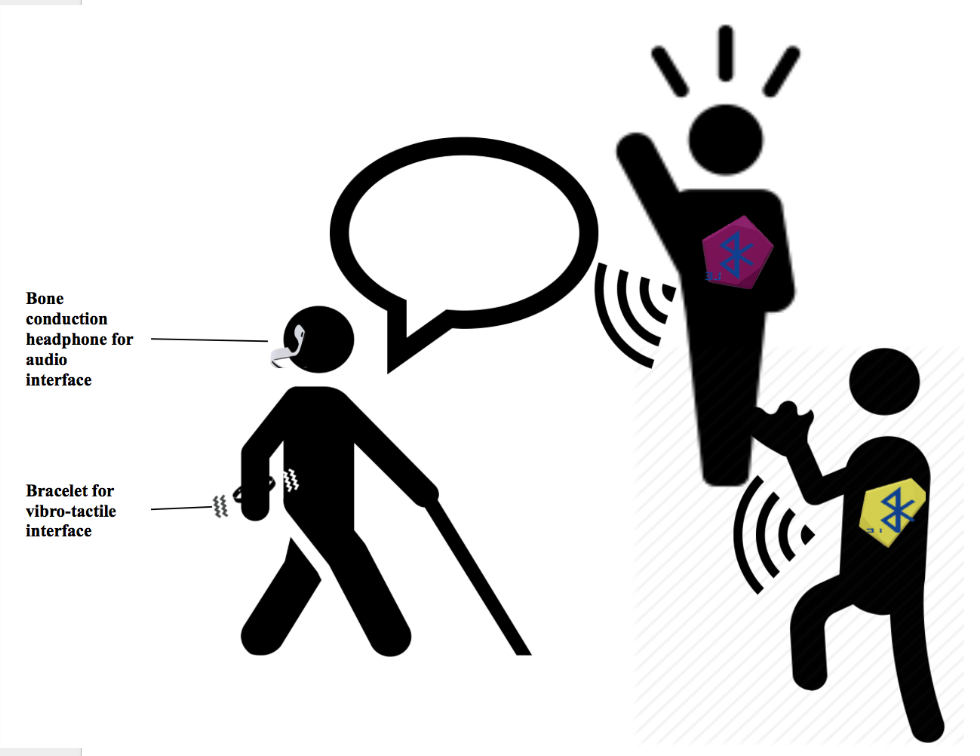
\includegraphics[width=\columnwidth]{figures/Proto2.png}
\end{center}
\caption{Interaction between user and other people in their surroundings}
\label{fig:system}
\end{figure}

\subsection{Bluetooth Low Energy Beacons}
To address the issue of identifying and placing moving persons in our environment, we use low-cost Estimote\footnote{https://estimote.com/} Bluetooth Low Energy beacons. People in the environment wear or carry the beacons.  In software, we map beacon ids to names of the assigned people.  In this way, beacons serve the same purpose as nametags do for a sighted person.  They broadcast their wearers' identity as a signal that can be picked up by the user's Bluetooth signal receiver to know who the person is.

Additionally, the beacons report distances with an accuracy that enables us to map to the distinct interpersonal proximity zones fairly well, allowing us to differentiate between people in the personal, social and public space of the user, so that information can be communicated to the user along with the identity.  Figure \ref{fig:beacon}\footnote{http://www.businessinsider.com/beacons-and-ibeacons-create-a-new-market-2013-12} shows what a Bluetooth beacon looks like.

\begin{figure}[htbp]
\centering
\begin{center}
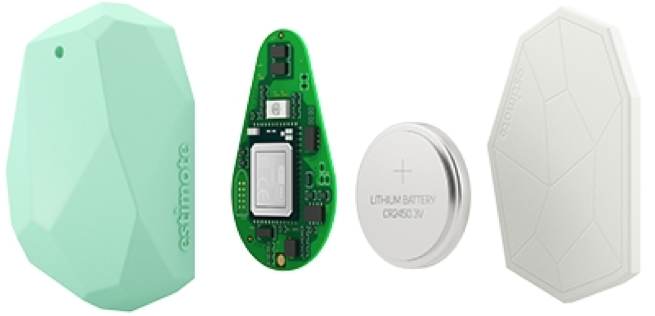
\includegraphics[width=\columnwidth]{figures/ble_hardware.png}
\caption{Bluetooth beacon} 
\label{fig:beacon}
\end{center}
\end{figure}


\subsection{The Wearable Device}
Inspired by the talking wristwatch worn by our user, we decided to embed our single-purpose device in a wrist-based wearable.
This wrist bracelet holds the Bluetooth receiver and transmitter, processing and memory unit, a vibro-tactile interface, and a button to control speech notifications. It has a counterpart Bluetooth bone conduction headphone which serves as the audio interface providing both speech notifications and sonifications. We chose to use a bone-conduction headphone so that we can provide audible notifications without requiring the user to wear earbuds that would block sound coming from the environment, which is important for the user to build their mental map of the environment. The bone-conduction headphone also ensures a level of privacy since the sound is transmitted by vibrations, and thus not audible to other people nearby.

Figure \ref{fig:wearable} shows the device being worn, Figure \ref{fig:insides} shows the internals of the device, and Figure \ref{fig:schematic} contains the schematic.

\begin{figure}[htbp]
\centering
\begin{center}
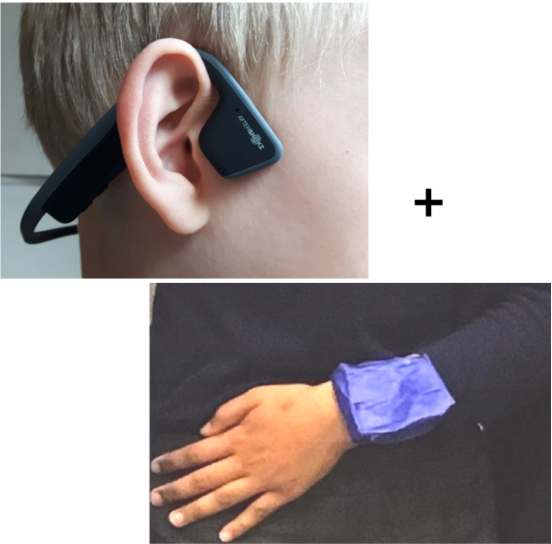
\includegraphics[width=.75\columnwidth]{figures/W.png}
\end{center}
\caption{Wearable}
\label{fig:wearable}
\end{figure}

\begin{figure}[htbp]
\centering
\begin{center}
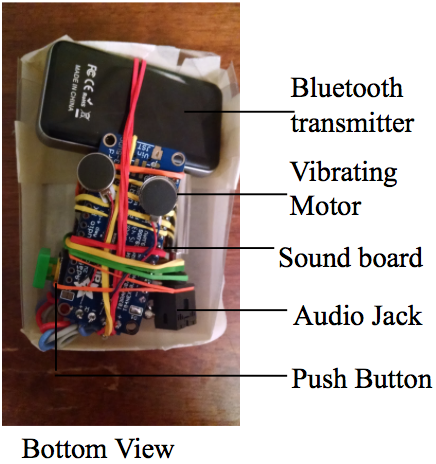
\includegraphics[width=.6\columnwidth]{figures/labeled.png}
\end{center}
\caption{Wearable internals}
\label{fig:insides}
\end{figure}

\begin{figure}[htbp]
\centering
\begin{center}
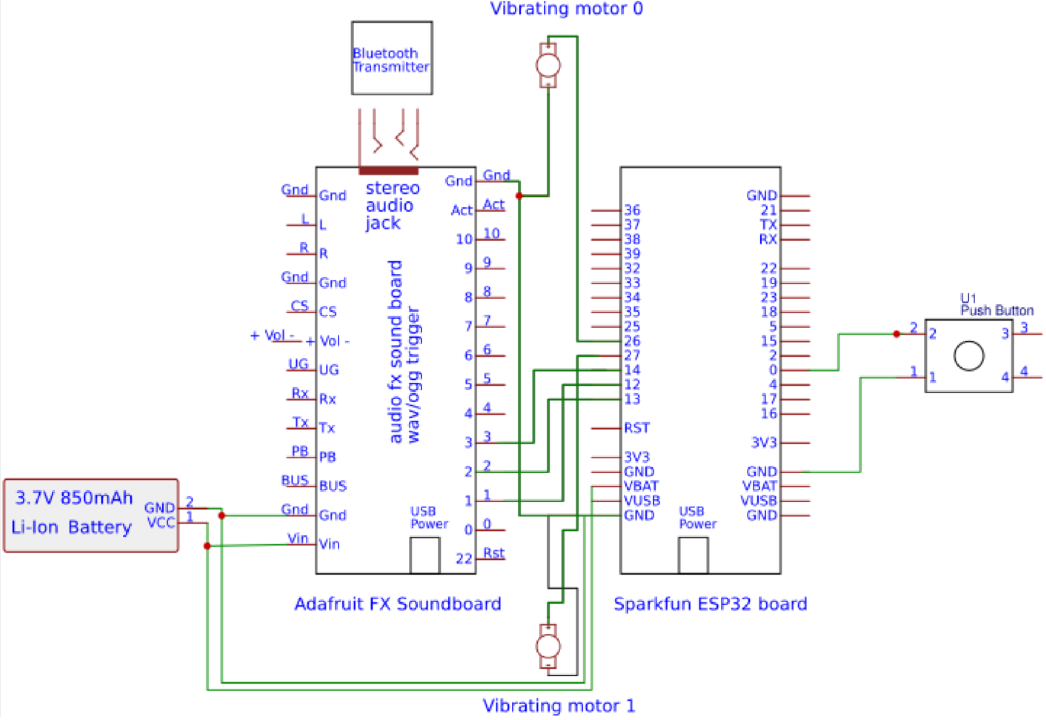
\includegraphics[width=1\columnwidth]{figures/schematic.png}
\end{center}
\caption{Wearable schematic}
\label{fig:schematic}
\end{figure}

For the primary processing and memory unit, we use the ESP32 chip as it is a small board with a built-in Bluetooth module that fits well on the user's wrist. The ESP32 chip has a Bluetooth Low Energy-compatible micro-controller, 30 input/output pins, and an FTDI FT231x, which converts USB to serial, and allows us to program the micro-controller from our computer. We power the ESP32 board using a Lithium-polymer battery to make it portable. There is also a mini-USB charging port which we used during most of the testing prototypes. 
 
To enable sonifications and speech notifications, we use the Adafruit FX Soundboard, which is about 1.9" x 0.85". It can store about 2MB worth of sound and can be powered by a 3-5V Lithium-Polymer battery. It has 11 triggers, enabling us to notify the user of 11 different events with different sounds. Since each user has 4 sounds (2 speech notification sounds,  2 sonifications) that are dedicated the device can convey information of about 3-4 people without cognitively overwhelming the user with too many different sounds. It is relatively easy to learn to differentiate between and keep track of about 10-11 sounds \cite{Roder:2001aa,Kujala:1995aa,Abel:2004aa}. Therefore, this is perfect for our use case. Each of the distinct sounds stored in the Soundboard are triggered in response to events occurring in the user's environment as they are informed by signals from the ESP32 I/O pins. 
 
The sounds differ in amplitude and vibration as a person changes their location in the 3 proximity zones. The sounds become louder and higher in pitch when the person is closer to the user. Therefore, it is the loudest and has the highest pitch when a person is in immediate proximity, however it becomes fainter as the person moves from the immediate to near and then far proximity zones. 
 
The Adafruit Soundboard is connected to a 3.5mm Audio Headphone Jack. Since we want the sonifications to be conveyed via the Bluetooth bone-conduction headphones, we plug in a Bluetooth transmitter to this audio headphone jack. This way the sounds are transmitted to the bone conduction headphone, which is placed on the user's cheek bones. The sound vibrations are conducted into the user's inner ear through the bones of the skull.
 
The vibro-tactile interface is controlled by two motors connected to the ESP32 chip. The motors vibrate at 3 different frequencies depending on the proximity zone that they are in. The higher the frequency of vibration, the closer the person is. Therefore, the motors vibrate vigorously when the person is in the immediate zone and become fainter as a person walks to the near and far proximity zones. 

The total cost of building this device is about \$115, broken down as: \$20 for the Adafruit Sound Board, \$20 for the ESP32, \$5 including the audio jack, motors and the casing, \$50 for the Bluetooth bone-conduction headset, \$50 for 3-4 Bluetooth Low Energy beacons, and \$20 for the Lithium-Polymer battery.

\subsection{Software Implementation}

Having discussed the hardware and the interface, now let us discuss how the software was developed. Since we were programming the ESP32 board directly, we used the Espressif Internet of Things (IoT) Development Framework (IDF) from the command line by connecting to the board using USB to establish a serial connection with the board.  The program was coded in C++. 

We used the Eddystone URL BLE protocol to give maximum flexibility as Eddystone URL packets can be received and processed by any Bluetooth receiver.

We developed an algorithm for ranging the beacons and classifying them into the different proximity zones. When BLE beacons's Eddystone URL packet  is received by the ESP32 board (that is, a person is detected nearby), the program notes the unique identity (URL) of the beacon and begins ranging.  

First, to determine proximity zone based on the Received Signal Strength Indication (RSSI), the program sorts the beacons from the closest (strongest RSSI) to the farthest (weakest RSSI) and classifies each beacon into a proximity zone (either immediate, near, far, or unknown). Second, to identify the person the program looks up the URL-Name pair from the hashtable.  

The timings of the scans are set to coincide with the frequency at which the beacon is transmitting. Our program is currently set to scan about every 4 seconds which is when the beacons are also set to broadcast. Additionally, the program is built to handle possible errors and scan failures.

Once the program categorizes the identity and the proximity of a beacon, it sets the pins that correspond to the particular sounds on the sound board and vibrational patterns of the motors to turn on and produce the respective sounds and vibrational patterns. This all happens in near real-time. Therefore, the user is notified shortly after the signal is received from the beacon. While the sonifications and the haptic notifications are reported to the user in near real-time, the speech notifications are only reported when the user asks to know exactly who is in their surroundings. There is a push button that the user can press to ask the device who is in their surroundings. Then, the device will accordingly produce the speech notification with the name of the person. If there are multiple people in the user's surroundings, the potential interactors are announced in a nearest to farthest order. The user interface only notifies the user when there is a change from the previous state. The program stores the information from the past three scans and only reports if there is a significant change in the proximity zone during this time. This is to prevent overwhelming the user with a constant stream of speech notifications, which could interfere with conversations or other activities the user is engaged in. 



\section{Evaluation}
\label{sect:evaluation}
We had several evaluation studies for the many iterative prototypes developed through the design thinking process. We tried to get feedback from a diverse set of participants.

The first prototype, the early iPhone-based system, was evaluated with an 87-year-old woman with no light perception who had experienced late-onset blindness. We evaluated a different set of participants in the usability studies in this section. 

For the second prototype, we worked with two distinct group of potential users: early-onset and adult/late-onset blindness. This process is described in detail in this section.

We employed the think-aloud protocol to evaluate user feedback during usability testing and gain insight into the user's thoughts, feelings and comfort levels in real-time as they were performing structured social interaction tasks. Once they had completed the tasks, we interviewed them for their overall feedback on the device. 

\subsection{Usability Testing: User Feedback Round 1}

We first collected user feedback from a 20-year-old legally blind female with no light perception who had experienced early-onset blindness and was blind with little to no light perception. The social interaction tasks took place in an empty classroom over a period of an hour. She had a guide dog to help her navigate the space.  
%Her usability testing results are reported in Figure 23. 

% \begin{figure}[!htbp]
%   \centering
%   \caption{Usability Testing Prototype 2: Tracking Independence in Task Performance in a classroom by a potential user}
%   \includegraphics[width=5in, height=6in]{user1.png}
%   \includegraphics[width=5in]{legend.png}
% \end{figure}

Overall, this user was very comfortable using the device to identify people as well as locate them in her space. She very quickly learned and adapted to the user interface. She was able to distinguish between the different proximity zones fairly well. She liked the idea of only having the identities announced when she pushed the button "Having this [pointing to the button] is so good. I would only want to know when [I] maybe enter a room" 
 
During the tasks, she performed well on all tasks and required no external assistance in maintaining and modulating a conversation as both the researcher and the potential interactor moved in the environment.
 
For possible improvements, she suggested that the voice was speaking rather slowly and loudly. "The sounds could be fainter." Additionally, she mentioned that having the vibrations and the sounds at the same time was like "saying the same thing twice". She would have liked to have either the haptic notifications or the sonifications and "have a button to switch between that".  We also discussed  her concern of how it would be a distraction during a class. "Can I like switch the sounds off when I'm in class?". 
 
Talking about the wearable, she said that it was still rather bulky and not really "fashionable", particularly because the headphones are very noticeable. She initially also had a little trouble moving around the space during the structured tasks, though, she used her dog to help navigate her surroundings. Generally, she said that the device would help her if she "did not know people in a new place".

% \textbf{Sociability and Technological Comfort Pre-Post Results}

% Paired samples t-tests were conducted to examine the potential difference in sociability and technological comfort between before and after using the assistive device. (Figure 24) The user experienced a marginally significant (\textit{p}= 0.048) improvement in sociability reported after the use of the assistive device (\textit{M}= 4.22, \textit{SD}= 1.27) compared to before the use of the assistive device (\textit{M}= 4.8, \textit{SD}=1.03). 
% % \begin{figure}[!htbp]
% %   \centering
% %   \caption{Graph showing the user's level of sociability before and after use of Prototype 2}
% %   \includegraphics[width=4in]{graph1.png}
% % \end{figure}

% There was not, however, a significant change in the level of technological comfort after the use of the assistive device (\textit{M}= 4.63,\textit{SD}= 1.03) compared to before the use of the assistive device (\textit{M}= 4.80, \textit{SD}=1.03; \textit{p} = 0.41). In fact, each of the statements on the scale were scored the same way. This might be because the user already was comfortable with technology use as well as learning new technical skills. (Figure 25)
% % \begin{figure}[!htbp]
% %   \centering
% %   \caption{Graph showing the user's level of technological comfort before and after use of Prototype 2}
% %   \includegraphics[width=4in]{graph2.png}
% % \end{figure}

% Overall, these tests showed that there was no change in the technological skills which remained high both before and after the interaction with the device. However, we noticed a slight improvement in sociability levels after just a one-hour session with the device. 

\subsubsection{Insights gained }
 
In summary, the user was successfully able to use the device to identify and place people in their surroundings. The user interface was easy to learn, and intuitive. On the other hand, we discovered the user's need to personally set their notification mode: vibration mode or sonification mode or even have a temporary off switch for when in high focus tasks that do not require social interactions. 
%There was also a marginally significant increase in the sociability levels of the user. 

\subsection{Usability Testing: User Feedback Round 2}

\begin{figure}[htbp]
  \centering
  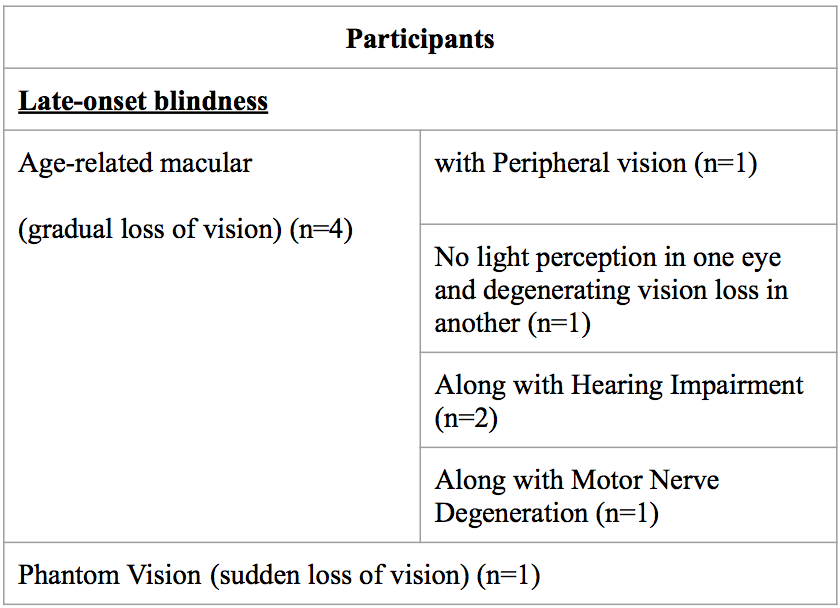
\includegraphics[width=\columnwidth]{figures/participants.png}
  \caption{Diversity in Participant Sample}
  \label{table:participants}
\end{figure}

Five participants (4 female, 1 male) were recruited from a nearby retirement community and assisted care facility. Participant ages ranged from 84 to 102 (\textit{M}=96, \textit{SD}=8.3). They had all experienced late-onset blindness: four are experiencing or have experienced gradual loss of vision due to age-related macular degeneration and one experienced sudden loss of vision due to a complication during cataract surgery causing phantom vision. All were legally blind. 

All participants had varied experiences adapting to their adult-onset blindness. One of them has no center vision but has good peripheral vision. Another participant is blind in one eye and is experiencing rapid vision degeneration in the other eye. The other participants have intersecting accessibility needs of not only being visually impaired, but also having hearing impairment and motor nerve degeneration. Table \ref{table:participants} summarizes the participants.

The usability studies were conducted over a period of two-and-half-hours. The users were able to recognize people in their surroundings even if they were far away and could not be seen or recognized at a distance. They were able to immediately use the device with minimal instruction suggesting that the device is easy-to-learn. After a quick demonstration,  they were even able to teach it to each other and perfectly explain the different features. The user interface did not seem to be overwhelming because it did not interfere in their conversations. If they wanted to know exactly who was there, they usually stopped speaking and pressed the button to hear the device speak but continued speaking regularly after. They also really liked that the headphone did not go into the ear but over it so that they could still hear other sounds from their surroundings. 

There was some uncertainty when potential interactors moved in and out of some rooms. Since the device announces only proximity of the potential interactor, they could be 'near' but still behind a wall or door. Furthermore, there was a lag if the room was small and/or the potential interactor moved rather quickly through space. 

Overall, everyone was able to perform the tasks successfully with no additional support and only relying on the device. Any additional support provided was only with regards to either how to wear the device initially. 
Figure \ref{fig:usability} summarizes the results from the usability testing.

\begin{figure}[!htbp]
  \centering
  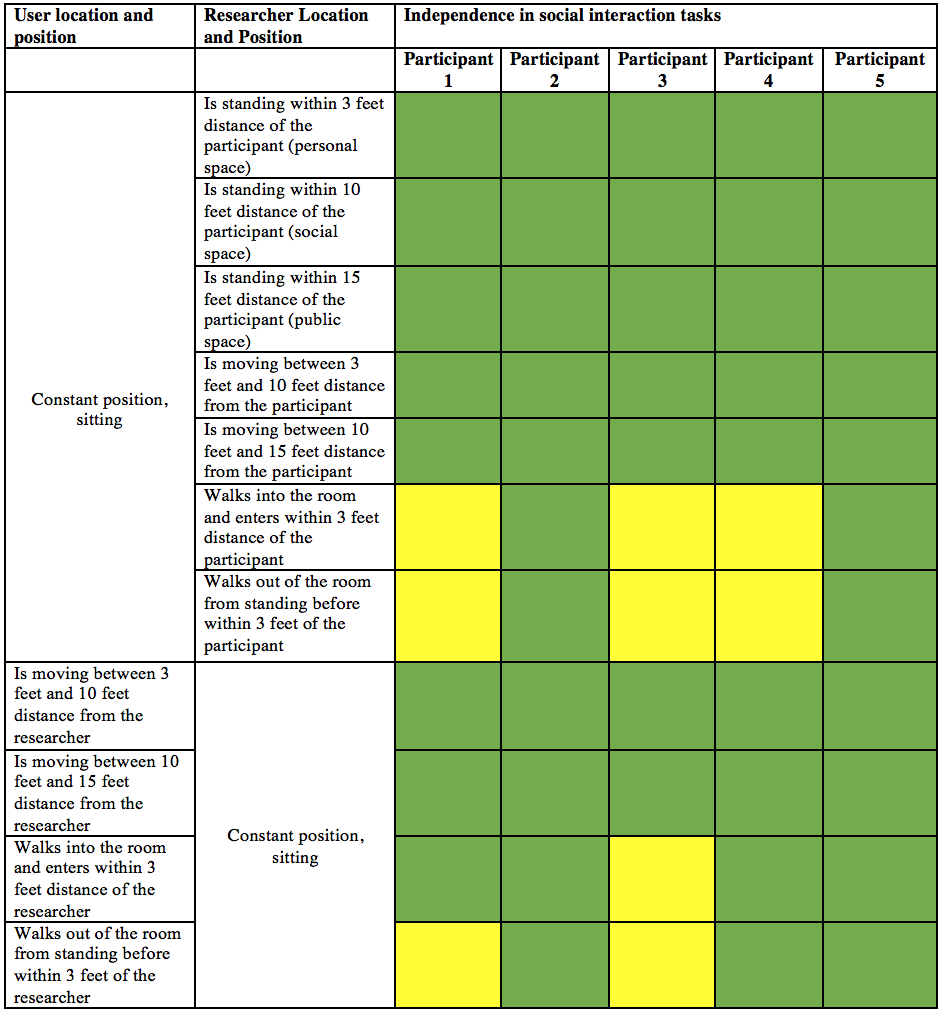
\includegraphics[width=\columnwidth]{figures/usability1.png}
  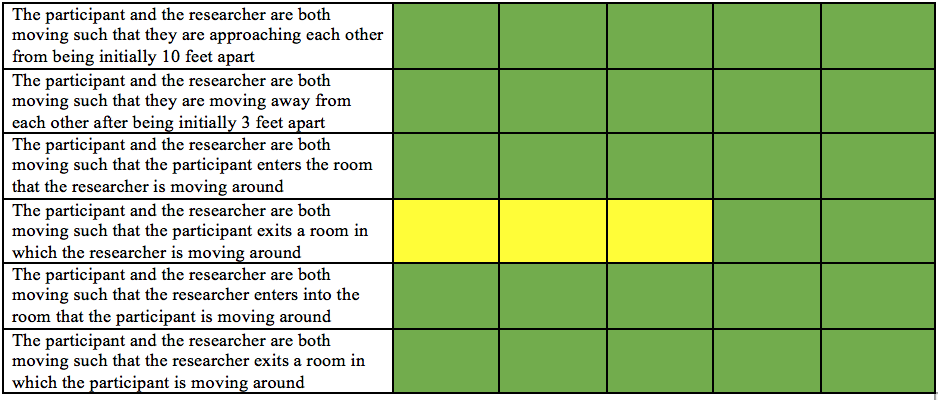
\includegraphics[width=\columnwidth]{figures/usability2.png}
  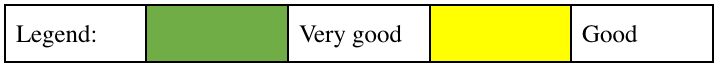
\includegraphics[width=2in]{figures/Legend.png}
  \caption{Usability Testing Prototype 2: Tracking Independence in Task Performance for 5 participants}
  \label{fig:usability}
\end{figure}

In conversations with the participants, we learned things beyond the social interaction tasks we asked them to do. 
They had some trouble putting on the strap of the wearable because it required a bit of dexterity to find the right hole to put the pin of the strap into. This was hard not only due to their reduced vision but also due to the motor dexterity required. They suggested that we replace the strap with "a thick elastic band or Velcro [that] could be easily snapped on". Another aspect of the wearable mentioned during potential improvements was that it is very bulky, particularly the headphones. Having something that they can wear around the ears "like earrings or for someone who does not wear earrings like [male participant], we can have something that goes over your glasses like an ear-piece behind the ear."
 
One of the users who is blind in one eye mentioned that it would be "helpful when there is further degeneration in the other eye" as well. As of now, he says, "since I am blind in this [left] eye, I would not have known who is there [points to his left field of vision] without moving my head completely so that my right eye could see. I can see a shape very indistinctly, but I would not know who it is if I was looking just straight ahead." 

Another participant who wears hearing aids, mentioned that she could still hear everything fine. This suggests that the hearing aids and these headphones do not interfere with each other. 
 
Additionally, some users mentioned possibly having just the vibration patterns because they did not need to be notified via sonifications in all environments and contexts. This seems to be consistent with our previous user study. However, one of the users with severe visual impairment and neuro-degeneration mentioned it was good to have both the sounds and the vibration patterns because if she missed the vibration pattern, she could still hear a sound notifying her. 

Discussing overall thoughts about the device at the conclusion of our user-feedback session, they said it was a "interesting device" that could easily be integrated into their daily routine. Even though many of them had some light perception, they said that the device was useful in making them more aware of other people who they would have otherwise missed. This would help them engage in conversations because they know more about the environment now than they did before. 

They also suggested many different applications in different contexts of their lives than just social interactions. One of the ideas was that it could be used as an added security measure where they can immediately know who is knocking at their door when they are not expecting someone. Another use was that it made them aware of someone near the puzzle area or near the gym, it would be easy to join them. 

% \textbf{Sociability and Technological Comfort Pre-Post Results}
 
% Paired samples t-tests were conducted to examine the potential difference in sociability and technological comfort between before and after using the assistive device. There was no significant change (\textit{p} = 0.72) in sociability reported after the use of the assistive device (\textit{M}= 3.60, \textit{SD}= 0.50) compared to before the use of the assistive device (\textit{M}= 3.04, \textit{SD}=1.12) by all the participants. However, one of the participants who had the most severe age-related macular degeneration with very little light perception reported a significantly higher level of sociability after using the device. (Figure 28)

% \begin{figure}[!htbp]
%   \centering
%   \caption{Graph showing each of the user's level of sociability before and after use of  assistive device}
%   \includegraphics[width=5in]{sociability.png}
% \end{figure}

% However, there was not a significant change in the level of technological comfort after the use of the assistive device (\textit{M}= 2.26, \textit{SD}= 1.02) compared to before the use of the assistive device (\textit{M}= 2.41, \textit{SD}=1.03). This might be because many of the participants reported very low levels of technological comfort. 

Even though the participants did not usually feel comfortable using technology,, they reported that they would be willing to learn new technology if it helped their vision. They also said that this particular device did not require them to know any high-level technology, so they felt comfortable using it.
%(Figure 29)

% \begin{figure}[!htbp]
%   \centering
%   \caption{Graph showing each of the user's level of technological comfort before and after use of assistive device}
%   \includegraphics[width=5in]{techcomfort.png}
% \end{figure}




\subsubsection{Insights gained}
 
In summary, the single-purpose wearable device was able to perform i1ts primary tasks of identifying people and letting the user know how far away the person is. The user interface was easy to learn, and intuitive. User feedback showed that we could improve the design by adding different modes: possibly vibration mode and sonification mode or even have a temporary off switch for when the user is engaged in high-focus tasks and does not want to engage in social interactions. 
%There was no significant change in the sociability levels or levels of technological comfort of the user during the short sessions we had. 

% \subsection{Overall Results}

% We employed a systems approach to inform our understanding of the user experience and building assistive technology and user interface by pulling from literature in cognitive neuroscience, sociology and technology. We put together a list of potential user’s requirements and product design requirements. 

% % \begin{figure}[!htbp]
% %   \centering
% %   \caption{Comparing the two prototype designs against the user needs and product requirements}
% %   \includegraphics[width=5in]{evaluation.png}
% % \end{figure}

% The first prototype’s design was informed by the literature review and was designed to fulfill these product requirement. When we performed usability testing and gathered user feedback we realized that the biggest positives from the iPhone-based prototype design was that it was a low-energy, durable solution that identified and placed individuals accurately in the user’s space. On the other hand, it was unintuitive, not easy-to-use and the user interface was rather cognitively overwhelming frustrating the user over a period of time.

% Since the device was not as usable as we expected, we looked to the devices that the potential users used successfully everyday. We realized that most of these devices were reliable and easy-to-use because they were single-purpose devices and we adjusted our understanding of the user experience and product requirements based on these insights gained.
 
% Our second prototype was  a single-purpose wearable device that conveyed to the user only the significant changes in proximity through sonifications, haptic notifications and speech notifications. Upon performing multiple rounds of usability testing and gathering user feedback, we observed that it was successful in not only informing the user of the right information - identity and proximity of the potential interactors, but also was successful in doing it in an easy-to-use, intuitive manner. 

% Observing the results we have seen through this project, we notice some overarching trends. First, the device is increasingly helping the user engage in social interactions without any additional support. Generally, most users have moved from being in the maximal or moderate assistance category to the no helper or modified dependence category on the independence scale. This shows that the device does help users independently engage in social interactions. Second, the user feedback has been overwhelmingly positive in terms of whether it helped them know who is in their surroundings. The marginal improvement in sociability levels even after just a short period of use shows that this device might have the potential over a period of time affect confidence in their interaction patterns.

% When compared with the iPhone design, there are two main things that the second design is not as good at. First, it is not as durable in its current iteration. If it falls or hits another surface, it is likely to break or not function properly. Second,  this second design is not capable of parallel processing. Since it can only do serial processing, the device might have some lag in detecting multiple beacon data and reporting them all. Not only does this device have a processing limitation, it also has a memory limitation in that its memory is smaller than that of an iPhone. Therefore, the second iteration can save only a certain number of sounds and notification patterns. This sets a limitation on the number of people we can beacon and the user can recognize that does not exist in the iPhone design. This is not a major problem currently, though it may be a concern as we scale the environments and contexts we want to map. 

\section{Conclusions and Future Work}
\label{sect:conclusion}
% * <blerner@mtholyoke.edu> 2018-09-12T16:10:26.784Z:
% 
% This is taken directly from the thesis and will need to be modified to fit the message of the paper.
% 
% ^.

\subsection{Lessons Learned}
This project shows us a way that we can overcome the challenges of socio-technical problems to contribute something significant to not only the field of assistive technology, but also to the field of multi-sensory augmentation in human-computer interaction.

While general human-computer interaction has been a topic that has been extensively studied by many disciplines, the visually-impaired or blind interaction with technology is a topic that is under- explored. As we are propelled into the fourth industrial revolution and an era of technology, this project expands on our understanding of how a significantly large group in our population interacts with technology. This project identifies challenges and defines possible solutions to better the visually- impaired or the aging populations' experience with technology.

Furthermore, this project begins to lay down the foundation for designing possible intuitive haptic and audio user interfaces that benefit the visually-impaired by understanding how they already interact with the world around them. We learned that it is easier and more intuitive for the visually-impaired to use single-purpose devices that they can definitely rely on for that single purpose. Instead of constant notification, only notifying them when there is a significant change in their environment or context works better. Having only one notification stream activated, either audio or haptic, at any given time helps augment their knowledge about their surroundings more effectively without overwhelming them.

Aspects of the design could also be used by other populations such as those with prosopagnosia - an inability to recognize faces, or those with depth perception problems, or even general memory issues such as dementia. This should possibly help them approach others to engage in social interactions more confidently. Conversely, many aspects could also be translated into possibly designing intuitive multi-sensory user interfaces for the sighted.

\subsection {Limitations}
While the current prototype's results are encouraging, there are a few limitations to this solution. Firstly, there is some improvement that needs to be made with regard to accurately reporting significant changes in position in real-time. There is still some uncertainty in situations where either the user is moving faster than the broadcasting or notification speed. For example, when a user presses the button when the potential interactor, Person A, is far, there will be a speech notification triggered which will say "Person A is far". However, if Person A has moved quickly from the far proximity zone to be immediately near the user before the speech notification has ended, this would be an incorrect notification. This is confusing because the user now believes that Person A is far, when in reality they are near. Possibly moving from the serial processing ESP32 board to a multi-thread processing system that can keep track of multiple information at the same time would help provide feedback in real-time. This is a limitation of the current prototype design.  

Secondly, we have to make trade-off between knowing who everyone in the surroundings is at any given point in time versus just knowing when a few important people are near you. In the current prototype design, it is computationally not possible to have more than about 3-4 people beaconed and detectable by the device. This is not a major limitation because it is also hard for the user to detect too many differences in notification patterns. It is especially hard to differentiate between haptic notifications because our sense of touch has a higher sensory threshold near the wrist. Furthermore, it will be harder for the user to resist sensory adaptation because not all the notifications will be as important. Also, if there are too many notifications, then it is hard to keep track of what each of them means or which ones are more important than the rest. Therefore, while this is not a major limitation because it would be cognitively overwhelming for the user, this limitation prevents this prototype device from scaling up to larger environments, and contexts.

Thirdly, this is a rather bulky device. This is because we are pulling different capabilities and functionalities from different hardware resources. This is a major limitation to the current prototype, however, if we were to engineer a board with Bluetooth transmitter and receiver functionality, micro-controller, sound storage, battery power it would be much simpler. We could also have the Bluetooth bone-conduction headphone designed to be much smaller. 

\subsection{Future Work}
It is imperative that we continue to explore these questions regarding use of assistive technology over a longer time period. In the current user studies, we had the users only use the device for less than an hour. This is a very short-trial period. Our observations showing that they were able to successfully use the device to perform the structured social interaction tasks, only shows that the device is easy-to-learn, easy-to-use and can help the user identify and place individuals on their cognitive map. 
%However, we were not able to study how the device answers the larger issue of loss of sociability, independence, and life satisfaction. This is because these are personality traits that only change over a period of time. 
From our observations, all we can tell is that this device has potential to improve the sociability, independence, and overall life satisfaction since the users were positive about its potential. This is a big question that needs to be explored. How does the assistive device affect sociability, personality, overall life satisfaction of the user over a period of time. Also, how does the relationship between the user and device develop? Do we see a change in reliability and trust built over a period of time?

On the other hand, having preliminarily explored how the visually impaired create mental maps and having leveraged this information to create our current audio-haptic user interface, we can further explore the sensory thresholds, sensory adaptation, mental imagery and mapping to design a better suited user interface based on different accessibility needs. For example, users with early-onset versus late-onset blindness might benefit from different user interfaces.  Similarly, some users also need accommodation for hearing loss.

Moreover, we could also explore how we can customize to these different accessibility needs. One way would be to have the user do an initial set-up to calibrate user needs as well as contextual and environmental needs. Another way, would be to build an intelligent user interface that learns the user's interaction patterns in different contexts and environments over a period of time and adapts accordingly.

In conclusion, having explored the cognitive and social basis of interaction and having built a technological solution that integrates into the user's existing schema, we are confident that technology can play a vital role in improving the experience of visually-impaired users and their interactions with other people in their surroundings.
\begin{acks}
\end{acks}


\bibliographystyle{ACM-Reference-Format}
\bibliography{whosthere}

\end{document}
